\documentclass[usenames,dvipsnames,svgnames,table,aspectratio=1610,mathserif]{beamer}

\mode<presentation> {

%\usetheme{default}
\usetheme{Madrid}

\setbeamertemplate{footline} % To remove the footer line in all slides uncomment this line

\setbeamertemplate{navigation symbols}{} % To remove the navigation symbols from the bottom of all slides uncomment this line
}

\usepackage{graphicx} % Allows including images
\usepackage{booktabs} % Allows the use of \toprule, \midrule and \bottomrule in tables
\usepackage{hyperref}
\usepackage{apacite}
\usepackage{fancyvrb}
\usepackage{color}
\usepackage{alltt}
\usepackage{listings}
\usepackage{framed}
\usepackage{courier}
\usepackage{minted}
\usepackage{epstopdf}
\usepackage{xifthen}
\usepackage[utf8]{inputenc}
\usepackage[T1]{fontenc}
\usepackage{textcomp}
\usepackage{gensymb}
\usepackage{svg}

\hypersetup{colorlinks=false}

\setbeamertemplate{bibliography entry title}{}
\setbeamertemplate{bibliography entry location}{}
\setbeamertemplate{bibliography entry note}{}
\setbeamertemplate{itemize items}[circle]
\setbeamertemplate{enumerate items}[circle]
\beamertemplatenavigationsymbolsempty
\setbeamertemplate{footline}{}

\newminted{haskell}{}
\newminted{java}{}
\newminted{scala}{}

\definecolor{g}{RGB}{0,100,0}
\newcommand{\highlight}[1]{\colorbox{yellow}{#1}}
\newcommand{\nega}[1]{\colorbox{yellow}{#1}}
\newcommand{\posi}[1]{\colorbox{green}{#1}}
\newcommand{\nl}{\vspace{\baselineskip}}
\newcommand{\pnl}{\pause \nl}

\graphicspath{{diagrams/}}

\newcommand{\textslide}[1]{{
\begin{frame}
\begin{center}

#1

\end{center}
\end{frame}
}}

\newcommand{\codeslide}[1]{{
\begin{frame}[fragile]
\begin{haskellcode}
#1
\end{haskellcode}
\end{frame}
}}

\newcommand{\imageslide}[2][1]{{
\begin{frame}\begin{center}
\includegraphics[scale=#1]{#2}
\end{center}\end{frame}
}}

\newcommand{\imageslideleft}[2][1]{{
\begin{frame}
\includegraphics[scale=#1]{#2}
\end{frame}
}}

\newcommand{\imagetextslide}[3][1]{{
\begin{frame}\begin{center}

{#3}

\includegraphics[scale=#1]{#2}
\end{center}\end{frame}
}}

\newcommand{\ctof}{{
\LARGE $\degree F = \degree C \times \frac{9}{5} + 32$
}}

\newcommand{\ftoc}{{
\LARGE $\degree C = (\degree F - 32) \div \frac{9}{5}$
}}

%%----------------------------------------------------------------------------------------
%	TITLE PAGE
%----------------------------------------------------------------------------------------

\title[Propagators]{Propagators: An Introduction} % The short title appears at the bottom of every slide, the full title is only on the title page
\titlegraphic{
\includegraphics[scale=0.2]{data61.eps}}
\author{George Wilson} % Your name
\institute[] % Your institution as it will appear on the bottom of every slide, may be shorthand to save space
{
Data61/CSIRO\\ % Your institution for the title page
\medskip
\href{george.wilson@data61.csiro.au}{george.wilson@data61.csiro.au} % Your email address
}
\date{\today} % Date, can be changed to a custom date

\begin{document}


%%%%%
%%%%% Intro section
%%%%%


\begin{frame}
\titlepage % Print the title page as the first slide
\end{frame}


\begin{frame}

\begin{columns}
  \begin{column}{0.5\textwidth}
    \begin{center}
      
\includegraphics[scale=0.015]{what-are-birds.jpg}

      \nl

      What?
    \end{center}
  \end{column}
  \begin{column}{0.5\textwidth}
    \begin{center}
      
\includegraphics[scale=0.3]{for-what-purpose.jpg}

      \nl

      Why?
    \end{center}
  \end{column}
\end{columns}

\end{frame}


%%%%%
%%%%% History
%%%%%


\begin{frame}

\begin{columns}
\begin{column}{0.5\textwidth}
Roots as early as the 1970's at MIT
\begin{itemize}
  \item Guy L. Steele Jr. 
  \item Gerald J. Sussman
  \item Richard Stallman
\end{itemize}

\nl

More recently:
\begin{itemize}
  \item Alexey Radul
\end{itemize}
\end{column}
\begin{column}{0.5\textwidth}

\begin{figure}
\centering
\def\svgwidth{\columnwidth}
\input{circuit.pdf_tex}
\end{figure}

\end{column}
\end{columns}

\end{frame}


\begin{frame}[fragile]

\begin{verbatim}
(define (map f xs)
  (cond ((null? xs) '())
        (else (cons (f (car xs))
                    (map f (cdr xs)))))))
\end{verbatim}
\end{frame}


\begin{frame}
\begin{columns}
\begin{column}{0.005\textwidth}
\end{column}
\begin{column}{0.4\textwidth}
And then
\begin{itemize}
\item Edward Kmett
\end{itemize}
\nl
\nl

\includegraphics[scale=0.2]{haskell.png}
\end{column}
\begin{column}{0.5\textwidth}
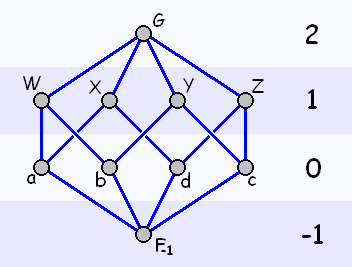
\includegraphics[scale=0.4]{hasse.png}

\nl
\nl

{\LARGE
  $x \le y \implies f(x) \le f(y)$
}
\end{column}
\end{columns}
\end{frame}


%%%%%
%%%%% What and why
%%%%%


\begin{frame}

\begin{center}
{\Huge Propagators}
\end{center}

\end{frame}


\begin{frame}
The {\it propagator model} is a model of computation

We model computations as {\it propagator networks}

\pnl

Propagator networks:
\begin{itemize}
\item are extremely expressive
\item lend themselves to parallel and distributed evaluation
\item allow different strategies of problem-solving to seamlessly cooperate
\end{itemize}
\end{frame}


\begin{frame}

A propagator network comprises
\begin{itemize}
\item cells
\item propagators
\item connections between cells and propagators
\end{itemize}

\end{frame}


\imageslide{cell1.pdf}
\imageslide{cell2.pdf}
\imageslide{prop.pdf}

%\imageslide{always1.pdf}
%\imageslide{always2.pdf}
%\imageslide{always3.pdf}
%\imageslide{always4.pdf}

\imageslide{upper1.pdf}
\imageslide{upper2.pdf}
\imageslide{upper3.pdf}

\imageslide{add1.pdf}
\imageslide{add2.pdf}
\imageslide{add3.pdf}
\imageslide{add4.pdf}


%%%%% bidirectionality


\begin{frame}
  \begin{center}
    \begin{LARGE}
      $z \leftarrow x + y$
    \end{LARGE}
  \end{center}
\end{frame}


\begin{frame}
  \begin{center}
    \begin{LARGE}
      $z = x + y$
    \end{LARGE}
  \end{center}
\end{frame}


\begin{frame}
  \begin{center}
    \begin{LARGE}
      $7 = x + 4$
    \end{LARGE}
  \end{center}
\end{frame}


\begin{frame}
  \begin{center}
    \begin{LARGE}
      $7 = 3 + 4$
    \end{LARGE}
  \end{center}
\end{frame}


\begin{frame}
  \begin{center}
    \begin{LARGE}
      $z = x + y$
    \end{LARGE}
  \end{center}
\end{frame}


\begin{frame}
  \begin{center}
    \begin{LARGE}
      $z \leftarrow x + y$

      \nl

      $x \leftarrow z - y$

      \nl

      $y \leftarrow z - x$

    \end{LARGE}
  \end{center}
\end{frame}


\imageslide{badd1.pdf}
\imageslide{badd2.pdf}
\imageslide{badd3.pdf}
\imageslide{badd4.pdf}


\begin{frame}
\begin{center}
{\LARGE Propagators let us express multi-directional relationships!}
\end{center}
\end{frame}

\imagetextslide[0.8]{celsius1.pdf}{\ctof}
\imagetextslide[0.8]{celsius2.pdf}{\ctof}
\imagetextslide[0.8]{celsius3.pdf}{\ctof}
\imagetextslide[0.8]{celsius4.pdf}{\ctof}
\imagetextslide[0.65]{celsius5.pdf}{\ctof \\ \nl \ftoc}
\imagetextslide[0.65]{celsius6.pdf}{\ctof \\ \nl \ftoc}
\imagetextslide[0.65]{celsius7.pdf}{\ctof \\ \nl \ftoc}
\imagetextslide[0.65]{celsius8.pdf}{\ctof \\ \nl \ftoc}
\imagetextslide[0.65]{celsius9.pdf}{\ctof \\ \nl \ftoc}
\imagetextslide[0.65]{celsius10.pdf}{\ctof \\ \nl \ftoc}
\imagetextslide[0.65]{celsius11.pdf}{\ctof \\ \nl \ftoc}
\imageslide[0.65]{celsius12.pdf}
\imageslide[0.65]{celsius13.pdf}
\imageslide[0.65]{celsius14.pdf}
\imageslide[0.65]{celsius15.pdf}
\imageslide[0.65]{celsius16.pdf}

\textslide{
\Large{We can combine networks into larger networks!}
}

\textslide{\Huge{?}}


%%%%% partiality


\textslide{\Large{Cells {\it accumulate information} about a value}}


\begin{frame}
\begin{center}
\Huge $[1,5]$
\end{center}
\end{frame}


\begin{frame}
\begin{center}
\Huge $[1, 5] \cup [2, 7] = [2,5]$

\pnl

\Huge $[2,5] + [9,10] = [11,15]$
\end{center}
\end{frame}


\begin{frame}

\end{frame}


\begin{frame}
\begin{center}
\Huge $\{True,\ False\}$
\end{center}
\end{frame}


\begin{frame}
TODO set intersection examples
\end{frame}


\imageslide[0.6]{doubleplus0.pdf}
\imageslide[0.6]{doubleplus1.pdf}
\imageslide[0.6]{doubleplus2.pdf}


\textslide{{\LARGE
What types are the values of the cells?
}}


\imageslide{cell1.pdf}
\imageslide{cell2.pdf}
\imageslide{cell3.pdf}
\imageslide{cell4.pdf}


%\begin{frame}[fragile]
%\begin{haskellcode}
%data Maybe a = Nothing | Just a
%\end{haskellcode}
%\end{frame}


%\imageslide{maybe1.pdf}
%\imageslide{maybe2.pdf}
%\imageslide{maybe3.pdf}
%\imageslide{maybe4.pdf}

%\imageslide[0.6]{doubleplus3.pdf}

%\imageslideleft{always1.pdf}

%\imageslideleft{always2.pdf}
%\imageslideleft{always3.pdf}
%\imageslideleft{always4.pdf}
%\imageslideleft{contradiction1.pdf}
%\imageslideleft{contradiction2.pdf}
%\imageslideleft{contradiction3.pdf}


\begin{frame}[fragile]
\begin{haskellcode}
data Perhaps a = Unknown | Known a | Contradiction
\end{haskellcode}
\end{frame}

\begin{frame}[fragile]

\begin{haskellcode}
data Perhaps a = Unknown | Known a | Contradiction
\end{haskellcode}

\nl

\begin{haskellcode}
instance Eq a => Monoid (Perhaps a) where

  mempty = Unknown

  mappend Unknown x           = x
  mappend x       Unknown     = x
  mappend Contradiction _     = Contradiction
  mappend _     Contradiction = Contradiction
  mappend (Known a) (Known b) =
    if a == b
      then Known a
      else Contradiction
\end{haskellcode}

\end{frame}


%\imageslideleft{contradiction4.pdf}
%\imageslideleft{contradiction5.pdf}
%\imageslideleft{contradiction6.pdf}
%\imageslideleft{contradiction7.pdf}
%\imageslideleft{contradiction8.pdf}
%\imageslideleft{contradiction9.pdf}

\imageslide[0.6]{doubleplus4.pdf}
\imageslide[0.6]{doubleplus5.pdf}
\imageslide[0.6]{doubleplus6.pdf}
\imageslide[0.6]{doubleplus7.pdf}
\imageslide[0.6]{doubleplus8.pdf}


\textslide{
\LARGE{
Is this the only type propagator cells can contain?

Will other monoids work?
}

\pnl

\Large{What about List?}
}

\imageslide[0.6]{doubleplus9.pdf}
\imageslide[0.6]{doubleplus10.pdf}
\imageslide[0.6]{doubleplus11.pdf}
\textslide{\Large{Looking good?}}
\imageslide[0.6]{doubleplus12.pdf}
\imageslide[0.6]{doubleplus13.pdf}
\imageslide[0.6]{doubleplus14.pdf}
\imageslide[0.6]{doubleplus11.pdf}
\imageslide[0.6]{doubleplus14.pdf}


\begin{frame}[fragile]
\begin{center}
\Large{
  We need commutativity!

  \nl

  $x \oplus y = y \oplus x$

  \pnl

  List append is not commutative!

  {\tt {
    [1,2,3] <> [4,5,6] == [1,2,3,4,5,6]
  }}

  {\tt {
    [4,5,6] <> [1,2,3] == [4,5,6,1,2,3]
  }}
}
\end{center}
\end{frame}


\textslide{\Large{
We need a commutative monoid

What about addition?

\nl

$x + y = y + x$
}}

\imageslide[0.6]{doubleplus15.pdf}
\imageslide[0.6]{doubleplus16.pdf}
\imageslide[0.6]{doubleplus17.pdf}

%% No good`
%\imageslide{badd5.pdf}
%\imageslide{badd6.pdf}
%\imageslide{badd7.pdf}
%\imageslide{badd8.pdf}
%\imageslide{badd9.pdf}
%\imageslide{badd10.pdf}
%\imageslide{badd11.pdf}


\textslide{\Large{
We need idempotence!

\nl

$x \oplus x = x$

}}

\textslide{\Large{

We need an idempotent, commutative monoid.

This structure is called a {\it join-semilattice}

\nl

Associativity

$(x \vee y) \vee z = x \vee (y \vee z)$
\nl

Commutativity

$x \vee y = y \vee x$
\nl

Idempotence

$x \vee x = x$

}}


\textslide{
{\LARGE Partial information that supports merging!}
}



\textslide{\LARGE Other examples?}

\end{document} 

